\documentclass[a4j,12pt,]{jarticle}
 \usepackage[dvipdfmx]{graphicx}
 \usepackage{float}
 \usepackage{siunitx} %%SI単位系用
 \usepackage{amssymb, amsmath}
 \usepackage{ascmac,here,txfonts,txfonts}
\usepackage{listings,jlisting}
\usepackage[dvipdfmx]{color}
\lstset{%
  language={Python},
  basicstyle={\small},%
  identifierstyle={\small},%
  commentstyle={\small\itshape\color[rgb]{0,0.5,0}},%
  keywordstyle={\small\bfseries\color[rgb]{0,0,1}},%
  ndkeywordstyle={\small},%
  stringstyle={\small\ttfamily\color[rgb]{1,0,1}},
  frame={tb},
  breaklines=true,
  columns=[l]{fullflexible},%
  numbers=left,%
  xrightmargin=0zw,%
  xleftmargin=3zw,%
  numberstyle={\scriptsize},%
  stepnumber=1,
  numbersep=1zw,%
  lineskip=-0.5ex%
}
\begin{document}

{\noindent\small 第3回報告書 \hfill\today}
\begin{center}
  {\Large CSVデータをElasticsearchサーバーに移行するプログラムの開発}
\end{center}
\begin{flushright}
  祖父江匠真 \\
\end{flushright}

\section{はじめに}
今回は, 道後小学校の既存PCにCSV形式で保存された太陽光発電の環境データ \cite{1}を, Elasticsearchサーバーに移行するプログラムを開発した.

\section{CSVデータをElasticsearchサーバーに移行するプログラムの開発}
今回, データ移行に使用したCSVデータの一部を図\ref{p1}に示す.
図\ref{p1}のCSVデータには, TIME, 日射強度, 外気温度, 直流電力, 交流電力のカラムが存在する.
なお, TIMEは計測日時であると推定される.

\begin{figure}[H]
  \begin{center}
    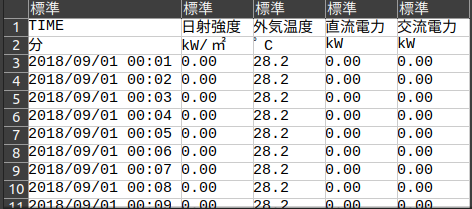
\includegraphics[width=160mm]{csv.png}
    \caption{移行元の太陽光発電の環境データ}
    \label{p1}
  \end{center}
\end{figure}

それぞれのカラムは, 現在リサイクル館から送信されている太陽光発電の環境データを保存するElasticsearchサーバーのインデックスにおける, JPtime, solarIrradiance(\si{\kilo}w/\si{\metre\squared}), airTemperature(\si{\degreeCelsius}), dc-pw(\si{\kilo}w), ac-pw(\si{\kilo}w)フィールドと対応する.

ソースコード\ref{sc1}は, 移行先となるElasticsearchサーバーのインデックスを作成するプログラムである.
既存のElasticsearchサーバーのインデックスとの互換性を考慮して, 今回開発する移行プログラムでインデックスに追加するドキュメントのフィールド名は, JPtime, solarIrradiance(\si{\kilo}w/\si{\metre\squared}), airTemperature(\si{\degreeCelsius}), dc-pw(\si{\kilo}w), ac-pw(\si{\kilo}w)としている.

\begin{lstlisting}[caption=CSVデータの移行先となるインデックスを作成するプログラム, label=sc1]
from elasticsearch import Elasticsearch

# Elasticsearchクライアント作成
es = Elasticsearch("http://localhost:9200")

# インデックス一覧の取得
indices = es.cat.indices(index="*", h="index").splitlines()
# 一度すべてのインデックスを削除する
for index in indices:
    es.indices.delete(index=index)

# マッピングを作成
mapping = {
    "mappings": {
        "properties": {
            "JPtime": {"type": "date"},
            "solarIrradiance(kw/m^2)": {"type": "float"},
            "airTemperature(℃)": {"type": "float"},
            "dc-pw(kw)": {"type": "float"},
            "ac-pw(kw)": {"type": "float"},
        }
    }
}
# マッピングを指定してインデックスを作成
es.indices.create(index="solars", body=mapping)

# 内部接続を閉じる
es.close()
\end{lstlisting}
ソースコード\ref{sc2}は,ソースコード\ref{sc1}で作成したインデックスにCSVデータを移行プログラムである.
Pythonのdatetimeモジュールで生成されるDateオブジェクトを, デフォルト設定のままElasticsearchに保存すると, Kibana上でUTC時間として扱われる.
更に, ブラウザ環境からタイムゾーンをAsia/Tokyoと推定し, 自動的にUTC時間からJST時間に変換するので9時間進んで表示されてしまう.
この現象の対策として, ソースコード\ref{sc2}の26行目では, Dateオブジェクトを作成する際に, JST時間に設定している.

\begin{lstlisting}[caption=CSV形式の太陽光発電データをElasticsearchサーバーに移行するプログラム, label=sc2]
from elasticsearch import Elasticsearch
import pandas as pd
import codecs
import datetime

# Elasticsearchクライアント作成
es = Elasticsearch("http://localhost:9200")

filepath = "data/DougoSyou/1809010000.csv"
with codecs.open(filepath, "r", "Shift-JIS", "ignore") as file:
    df = pd.read_csv(file, delimiter=",", skiprows=[1])

    for i, row in df.iterrows():
        year = int(row["TIME"][:4])
        month = int(row["TIME"][5:7])
        day = int(row["TIME"][8:10])
        hour = int(row["TIME"][11:13])
        minute = int(row["TIME"][14:])
        row = {
            "JPtime": datetime.datetime(
                year,
                month,
                day,
                hour,
                minute,
                tzinfo=datetime.timezone(datetime.timedelta(hours=9)),
            ),
            "solarIrradiance(kw/m^2)": float(row["日射強度"]),
            "airTemperature(℃)": float(row["外気温度"]),
            "dc-pw(kw)": float(row["直流電力"]),
            "ac-pw(kw)": float(row["交流電力"]),
        }
        es.create(index="solars", id=i + 1, document=row)

# 内部接続を閉じる
es.close()
\end{lstlisting}

ソースコード\ref{sc2}の実行によってインデックスに追加されたドキュメントを図\ref{p2}に示す.
図\ref{p2}より, ドキュメント数が43199であることが分かるが, 今回使用したCSVデータは2018年9月1日から2018年9月30日までの間, 1分ごとに計測されたデータであるので, 計測回数とドキュメント数が一致していることから, 全てのCSVデータを正しくElasticsearchサーバーに移行できたことが分かる.

\begin{figure}[H]
  \begin{center}
    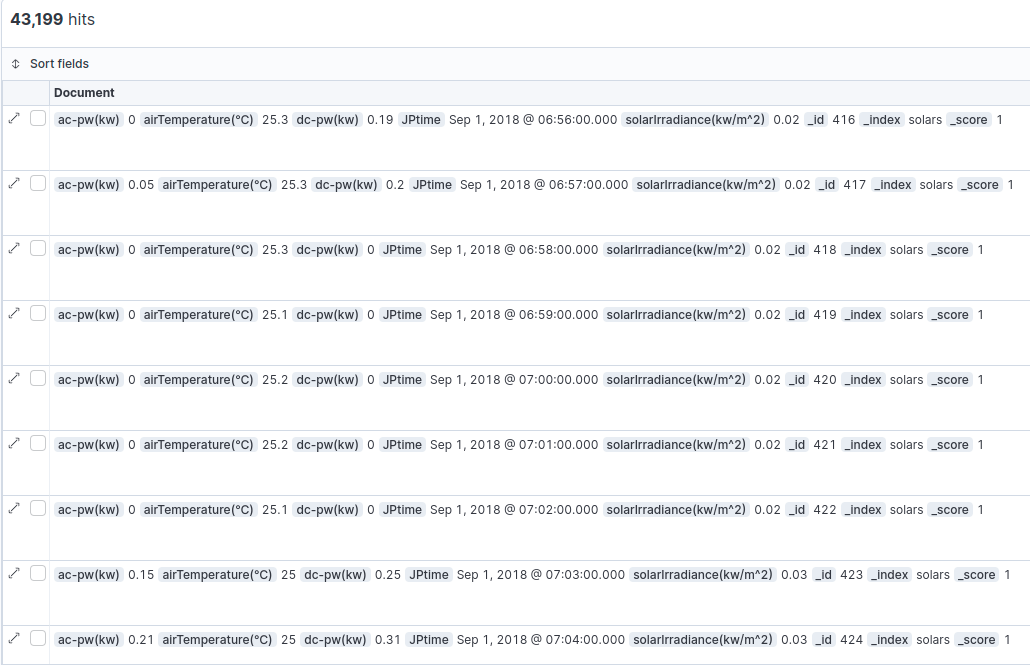
\includegraphics[width=160mm]{kibana.png}
    \caption{移行後の太陽光発電の環境データ}
    \label{p2}
  \end{center}
\end{figure}

\section{おわりに}
今回は, 道後小学校の既存PCにCSV形式で保存された太陽光発電の環境データを, Elasticsearchサーバーに移行するプログラムを開発した.
次回は, 道後小学校の既存PCにある全てのCSVデータをElasticsearchサーバーに移行するプログラムを開発する.

\begin{thebibliography}{5}
  \bibitem{1}都築,"道後小学校の既存PCに蓄積された観測データ",\\ http://gakunai.ee.ehime-u.ac.jp/~tsuzuki/study/SCOPE2014/ExistingPCdata/DougoSyou/,参照 May 16, 2022.
\end{thebibliography}

\end{document}